\section{Can geometric agreement be trusted?}
\label{sec:geometric-agreement}

\begin{figure}[!htb]
\centering
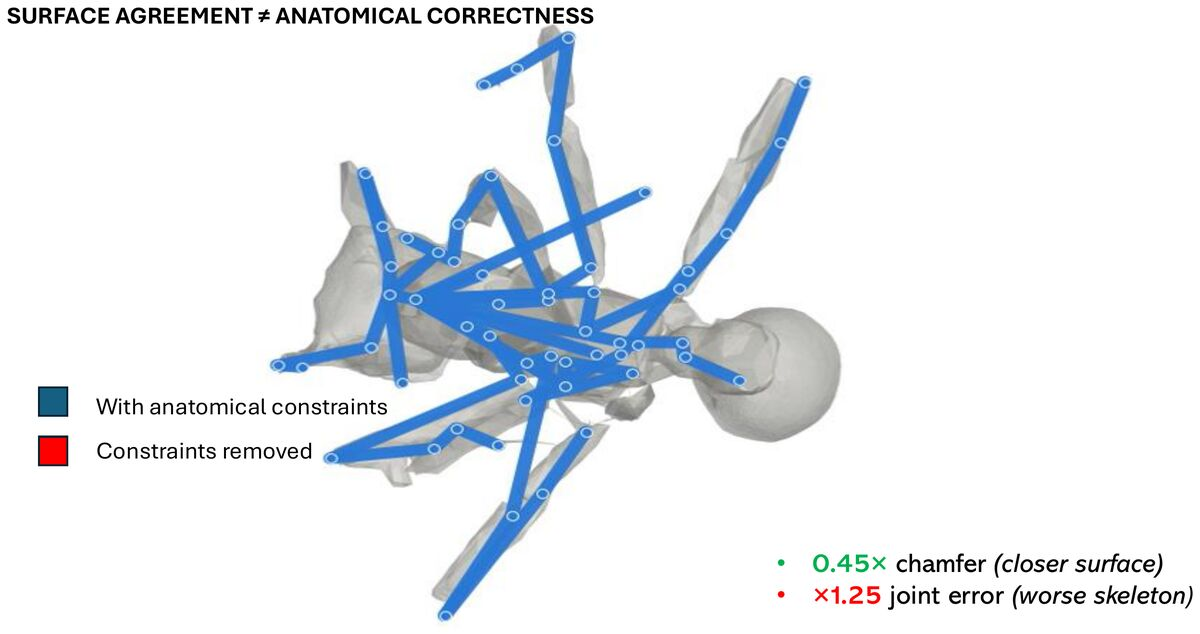
\includegraphics[width=0.58\linewidth]{figures/fig_geometric_agreement.jpg}
\caption{Removing anatomical (rotation-limit) constraints from the objective
moves surface distance and skeleton accuracy in \emph{opposite} directions:
the fit looks better by the metric the optimiser sees, and is worse by the
metric that matters. Skeleton overlay: blue, with anatomical constraints
active.}
\label{fig:geometric-agreement}
\end{figure}

\begin{investigation}{I3}{Is surface agreement a safe proxy for anatomical correctness?}
\invQuestion{If a fit's Chamfer distance improves, has the underlying
skeleton also become more accurate?}
\invMethod{Same specimen set, anatomical rotation-limit constraints toggled
on and off, Chamfer distance and joint-position error compared under each
configuration.}
\invResult{Removing constraints yields $0.45\times$ the Chamfer distance (a
closer surface) but $1.25\times$ the joint error (a worse skeleton): the
fit that scores better on the objective's own terms is the anatomically
worse one.}
\invVerdict{REJECT}{Surface-proximity metrics alone cannot adjudicate fit
quality. Confirms \F{F1}, independently of the rotation-probe and
10-specimen batch results referenced in the findings ledger
(\S\ref{sec:ledger}), and is the direct motivation for the two-tier
evaluation suite of \S\ref{sec:eval-suite}.}
\end{investigation}

The mechanism is not subtle once stated: every term in the registration
objective (\S\ref{sec:registration}) is a function of the two surfaces, and
none of them is a function of which point on the template surface is
supposed to represent which point on the target. A lower value of
$\mathcal{L}_{\mathrm{chamfer}}$ certifies that the fitted mesh covers the
target; it does not certify that vertex $i$ has landed on the anatomical
locus vertex $i$ is defined to represent. \S\ref{sec:skeleton-underdetermined}
traces this observation to a specific, structural property of the objective.
